\documentclass[12pt]{article}
\usepackage[margin=.5in]{geometry}
\usepackage{amsmath}
\usepackage{amsthm}
\usepackage{amsfonts}
\usepackage{amssymb}
\usepackage{mathtools}
\usepackage{float}
\usepackage{graphicx}
\usepackage{setspace}
\usepackage{epstopdf}
\usepackage{showframe}
\usepackage[utf8]{inputenc}
\usepackage[T1]{fontenc}
\usepackage{lmodern}

\newtheorem{assumption}{Assumption}
\newtheorem{lemma}{Lemma}

\DeclareMathOperator*{\argmin}{argmin}
\DeclareMathOperator*{\argmax}{argmax}

\begin{document}
% discrete messages
\section{discrete messages}
Assume throughout existence and uniqueness of solutions. 
% one if by land, two if by sea...
\subsection{one if by land, two if by sea...}
\onehalfspacing
For each $x\in[0,1]$, let the message $m_{x}:[0,1]\rightarrow\{m_{L},m_{H}\}$ be given by
\begin{equation*}
m_{x}(q)=\left\{\begin{array}{ll}
m_{L} & \text{if } q<x \\
m_{H} & \text{otherwise}
\end{array}\right.
\end{equation*}
and the action $A_{x}:\{m_{L},m_{H}\}\rightarrow\mathbb{R}$ by
\begin{equation*}
A(m)=\left\{\begin{array}{ll}
\argmin_{a}\:\int\limits_{0}^{x}{L(a-q)I(q)g(q)dq} & \text{if } m=m_{L} \\
\argmin_{a}\:\int\limits_{x}^{1}{L(a-q)I(q)g(q)dq} & \text{otherwise}
\end{array}\right.
\end{equation*}
where $L$, $I$ and $g$ are defined in the paper. The receiver's first-order conditions for $a_{L}:=A(m_{L})$ and $a_{H}:=A(m_{H})$ are
\begin{align*}
0&=\int\limits_{0}^{x}{L'(a_{L}(x)-q)I(q)g(q)dq};\\
0&=\int\limits_{x}^{1}{L'(a_{H}(x)-q)I(q)g(q)dq}.
\end{align*}
The sender chooses $x$ to minimize total loss:
\begin{equation*}
\min_{x}\:\int\limits_{0}^{x}{L(a_{L}(x)-q)I(q)g(q)dq}+\int\limits_{x}^{1}{L(a_{H}(x)-q)I(q)g(q)dq}.
\end{equation*}
The sender's first-order condition for $x$ is
\begin{align*}
0&=\int\limits_{0}^{x}{L'(a_{L}(x)-q)a_{L}'(x)I(q)g(q)dq}+L(a_{L}(x)-x)I(x)g(x)\\
&+\int\limits_{x}^{1}{L'(a_{H}(x)-q)a_{H}'(x)I(q)g(q)dq}-L(a_{H}(x)-x)I(x)g(x)
\end{align*}
Using the receiver's first-order conditions, we obtain
\begin{equation*}
L(a_{L}(x)-x)=L(a_{H}(x)-x).
\end{equation*}
$L(|\bullet|)$ is even and $L'>0$, so there are two solutions: $a_{L}(x)=a_{H}(x)$ and $x=(a_{L}(x)+a_{H}(x))/2$. Assume (correctly, I think) that the second solution is the unique minimizer of the total loss. $a_L$, $a_{H}$ and $x$ obey
\begin{align*}
0&=\int\limits_{0}^{x}{L'(a_{L}-q)I(q)g(q)dq}\\
0&=\int\limits_{x}^{1}{L'(a_{H}-q)I(q)g(q)dq}
\end{align*}
and
\begin{equation*}
x=\frac{a_{L}+a_{H}}{2}.
\end{equation*}
There are three equations and three unknowns. 
% example
\subsubsection{example (in progress)}
Let $L(x)=\frac{1}{2}x^2$, $I(x)=b+(1-2b)x$, and $g(x)=1$.
\begin{figure}[H]
\centering
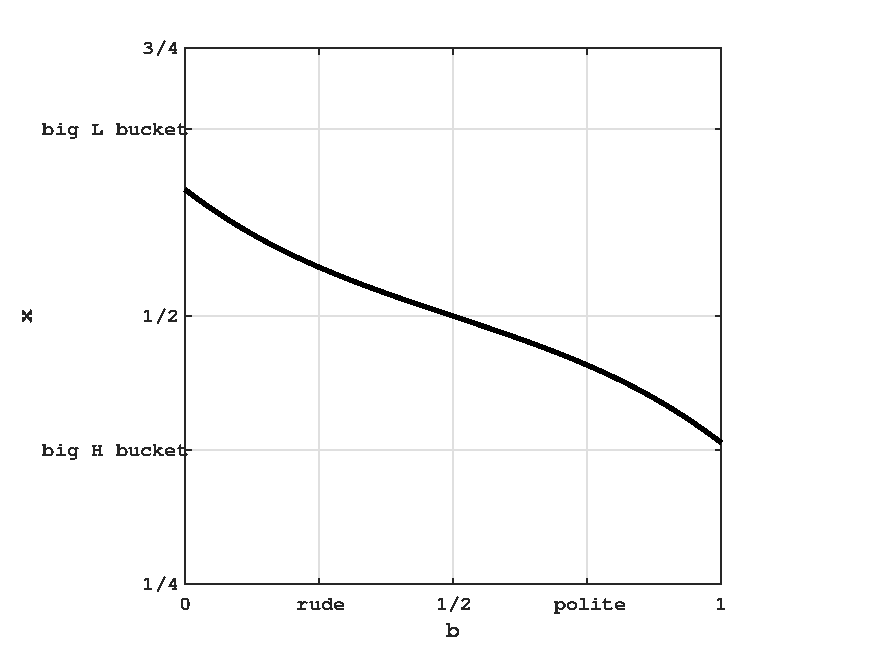
\includegraphics{example1}
\caption{$L(x)=.5x^2$, $g(x)=1$ and $n=2$.}
\end{figure}

\begin{figure}[H]
\centering
\begin{tabular}{c}
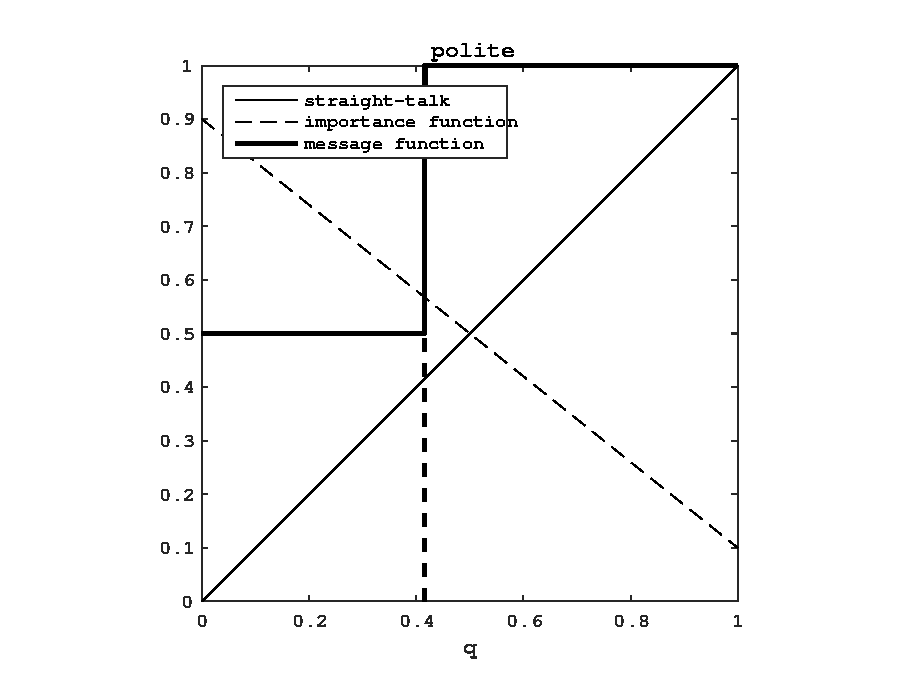
\includegraphics{polite2} \\
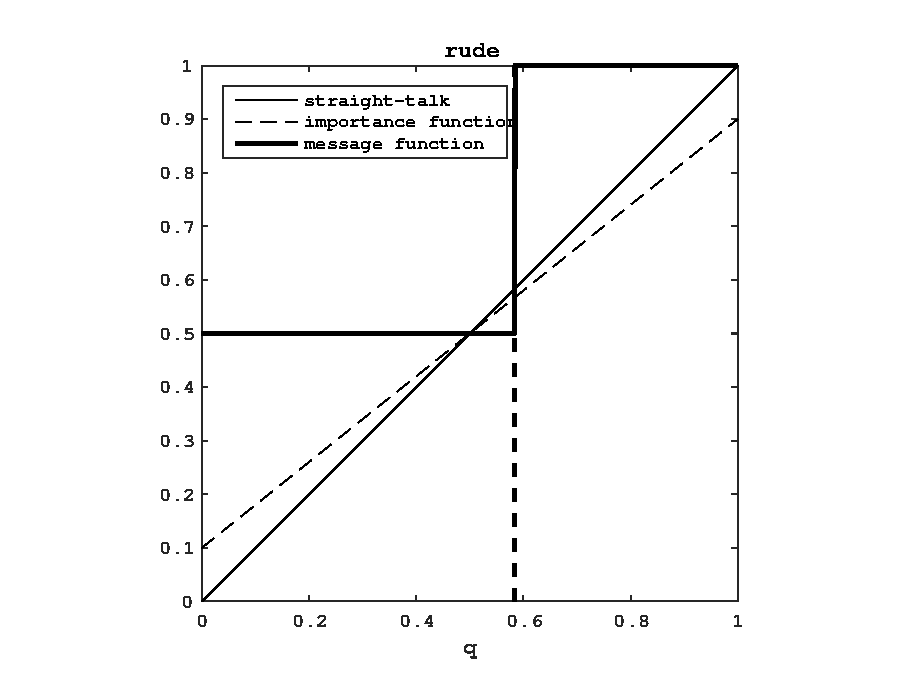
\includegraphics{rude2}
\end{tabular}
\caption{$L(q)=.5q^2$, $I_{rude}(q)=.1+.8q$, $I_{polite}(q)=.9-.8q$, $g(q)=1$ and $n=2$.}
\end{figure}
\begin{figure}[H]
\centering
\begin{tabular}{c}
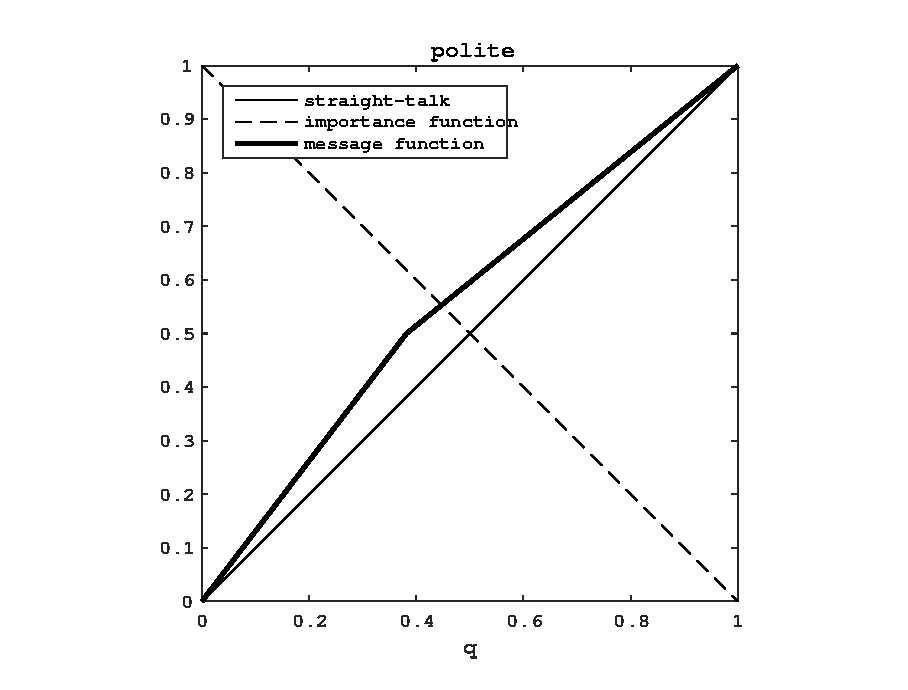
\includegraphics{polite2v1} \\
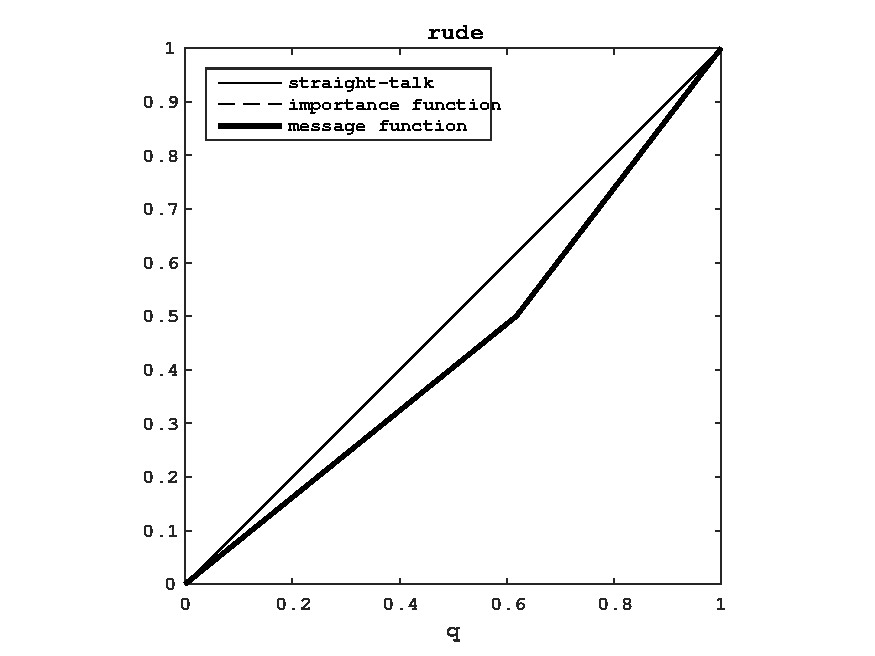
\includegraphics{rude2v1}
\end{tabular}
\caption{$L(q)=.5q^2$, $I_{rude}(q)=.1+.8q$, $I_{polite}(q)=.9-.8q$, $g(q)=1$ and $n=2$.}
\end{figure}
% ...three if by air?
\subsection{...three if the British are drinking tea}
Let there be $n\in\mathbb{N}$ messages: $m_{1},m_{2},\ldots,m_{n}$. For each partition $P=\{x_{0},x_{1},\ldots,x_{n}\}$ of $[0,1]$ with $0=x_{0}<x_{1}<\cdots<x_{n}=1$, let the message $m_{P}:[0,1]\rightarrow\{m_{1},m_{2},\ldots,m_{n}\}$ be given by
\begin{equation*}
m_{P}(q)=\sum_{t=1}^{n}m_{t}\chi_{[x_{t-1},x_{t})}(q)+m_{n}\chi_{\{1\}}(q)
\end{equation*}
and the action $A_{P}:\{m_{1},m_{2},\ldots,m_{n}\}\rightarrow[0,1]$ by given by
\begin{equation*}
A_{P}(m)=\sum_{t=1}^{n}\argmin_{a_{t}}\:\chi_{\{m_{t}\}}(m)\int\limits_{x_{t-1}}^{x_{t}}{L(a_{t}-q)I(q)g(q)dq}
\end{equation*}
where $\chi$ is the indicator function and $L$, $I$ and $g$ are defined in the paper. Fix $t\in\{1,2,\ldots,n\}$. The receiver's first-order condition for $a_{t}:=A(m_{t})$ is 
\begin{equation*}
0=\int\limits_{x_{t-1}}^{x_{t}}{L'(a_{t}(x_{t},x_{t-1})-q)I(q)g(q)dq}.
\end{equation*}
The sender chooses $P$ to minimize total loss:
\begin{equation*}
\min_{P}\:\sum_{t=1}^{n}\:\int\limits_{x_{t-1}}^{x_{t}}{L(a_{t}(x_{t},x_{t-1})-q)I(q)g(q)dq}.
\end{equation*}
The sender's first-order condition for $x_{t}$ is
\begin{align*}
0&=\int\limits_{x_{t-1}}^{x_{t}}{L'(a_{t}-q)\frac{\partial a_{t}}{\partial x_{t}}I(q)g(q)dq}+L(a_{t}-x_{t})I(x_{t})g(x_{t})\\
&+\int\limits_{x_{t}}^{x_{t+1}}{L'(a_{t+1}-q)\frac{\partial a_{t+1}}{\partial x_{t}}I(q)g(q)dq}-L(a_{t+1}-x_{t})I(x_{t})g(x_{t})
\end{align*}
so that
\begin{equation*}
L(a_{t}-x_{t})=L(a_{t+1}-x_{t}).
\end{equation*}
Again, there are two solutions: $a_{t}=a_{t+1}$ and $x_{t}=(a_{t}+a_{t+1})/2$. Assume that the second solution is the unique minimizer of the total loss. $a_{1},a_{2},\ldots,a_{n}$ and $x_{1},x_{2},\ldots,x_{n-1}$ obey
\begin{equation*}
0=\int\limits_{x_{t-1}}^{x_{t}}{L'(a_{t}-q)I(q)(q)dq}
\end{equation*}
for $t\in\{1,2,\ldots,n\}$ and 
\begin{equation*}
x_{t}=\frac{a_{t}+a_{t+1}}{2}
\end{equation*}
for $t\in\{1,2,\ldots,n-1\}$. There are $2n+1$ equations and $2n+1$ unknowns.
\begin{figure}[H]
\centering
\begin{tabular}{c}
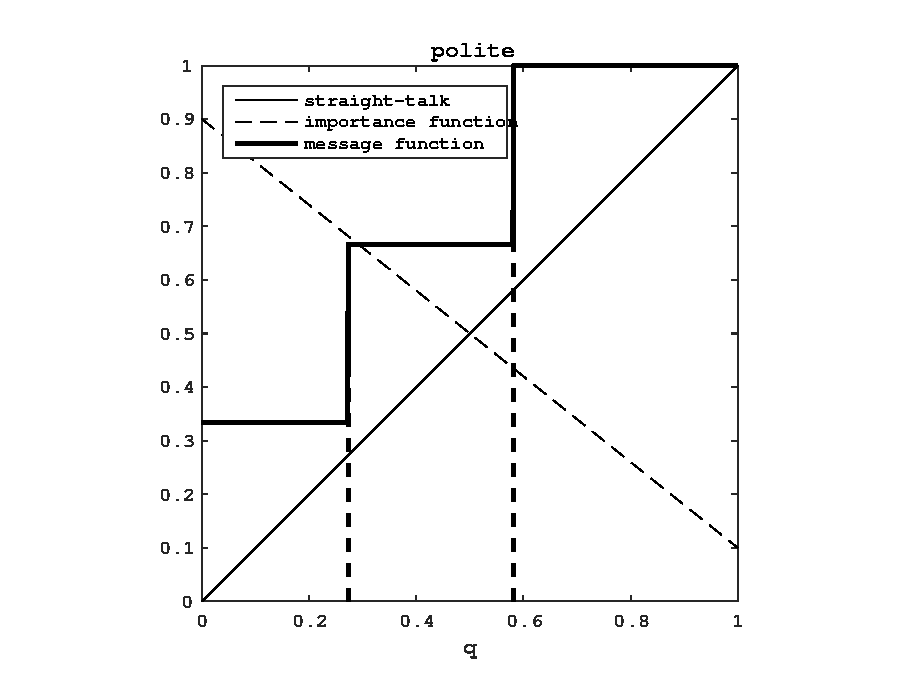
\includegraphics{polite3} \\ 
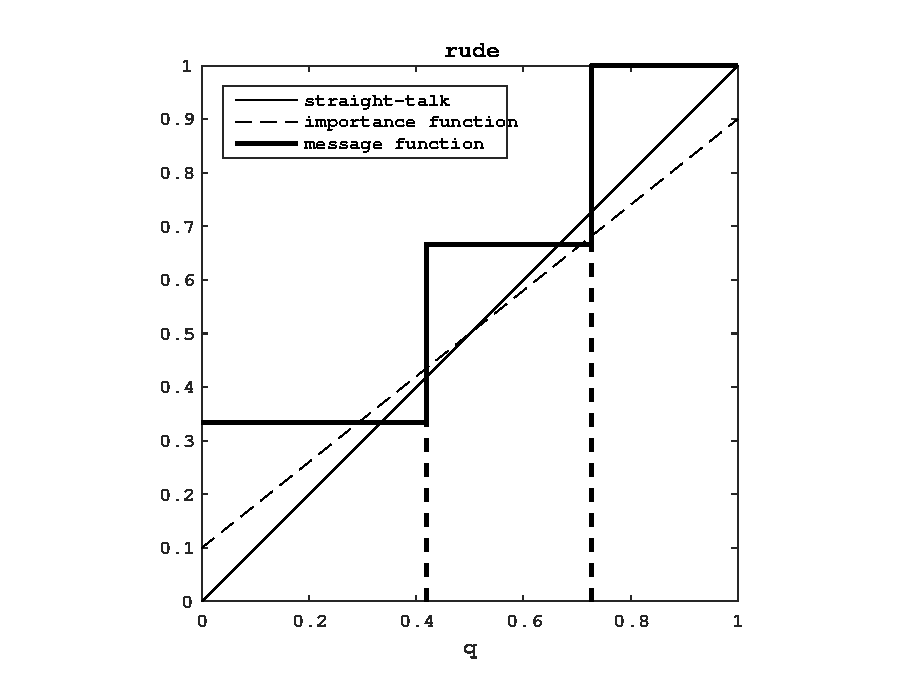
\includegraphics{rude3}
\end{tabular}
\caption{$L(q)=.5q^2$, $I_{rude}(q)=.1+.8q$, $I_{polite}(q)=.9-.8q$, $g(q)=1$ and $n=3$.}
\end{figure}
\begin{figure}[H]
\centering
\begin{tabular}{c}
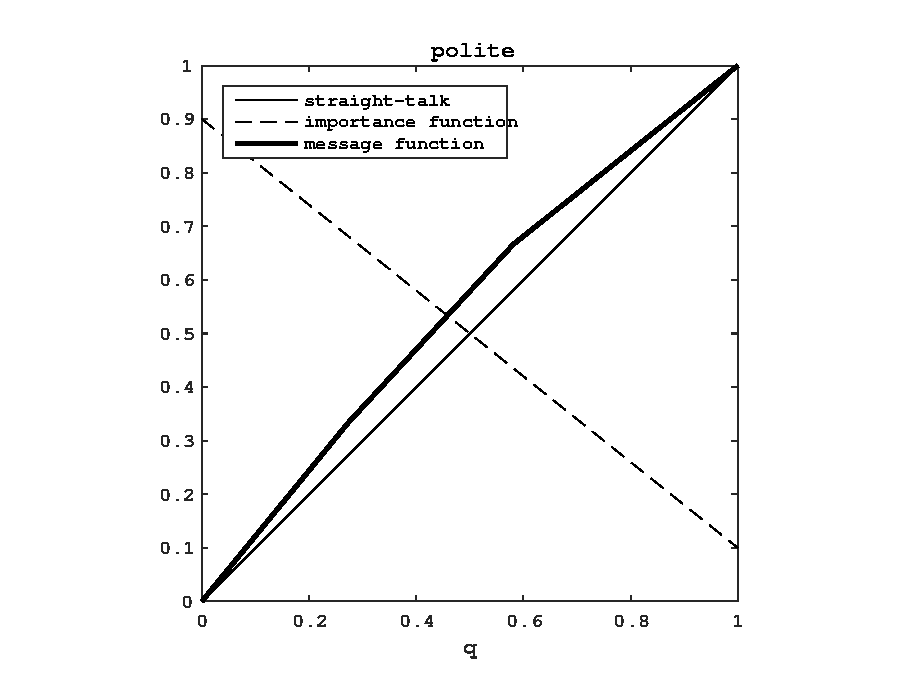
\includegraphics{polite3v1} \\ 
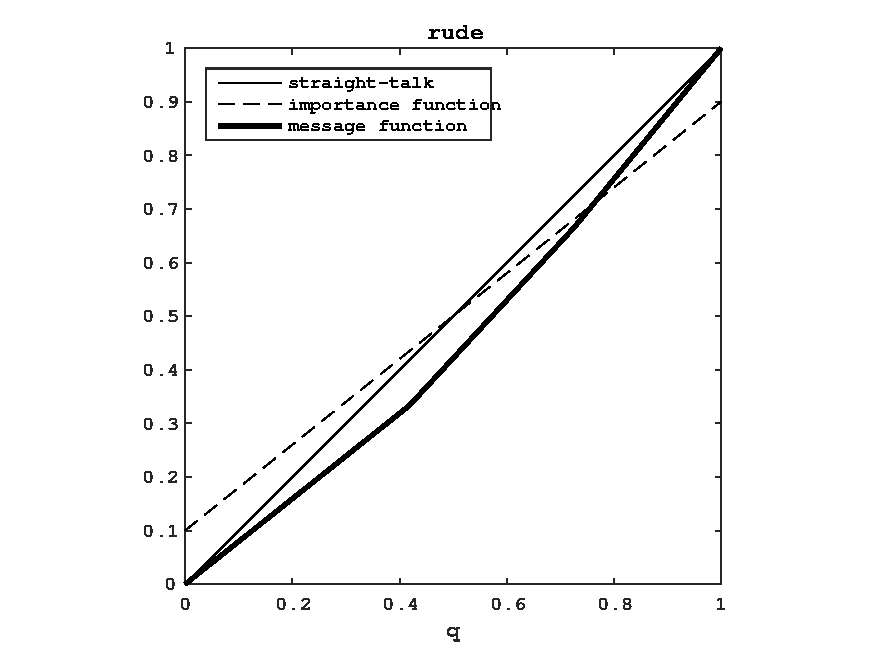
\includegraphics{rude3v1}
\end{tabular}
\caption{$L(q)=.5q^2$, $I_{rude}(q)=.1+.8q$, $I_{polite}(q)=.9-.8q$, $g(q)=1$ and $n=3$.}
\end{figure}
\end{document}
